\chapter{Compression and Generalization: PAC-Bayes and MDL}

\section{From Learning to Generalization: The Central Question}
%==========================

Let's start by clarifying what we mean by generalization and why it's the central challenge in machine learning. The setup is simple to state but profound in its implications.

\vspace{0.3cm}

You have a training dataset of examples drawn from some unknown distribution. You use this dataset to learn a model---perhaps a neural network, perhaps something simpler. The model performs well on the training data, achieving low loss. But what you really care about is how well the model performs on new data drawn from the same distribution. This gap between training performance and test performance is the generalization gap, and understanding it is the key to building reliable systems.

\vspace{1em}

\subsection{The Overfitting Trap}

Here's why generalization is hard. Suppose you have a training dataset with one thousand examples, and you want to learn a binary classifier. You could memorize all one thousand examples perfectly, achieving zero training error. But this memorization tells you nothing about how to classify the thousand-and-first example. You've learned the training data, but you haven't learned the underlying pattern.

\vspace{0.3cm}

Modern neural networks make this problem more acute because they have enormous capacity. A large language model with billions of parameters could, in principle, memorize vast amounts of training data. And yet, these models do generalize. They learn patterns that transfer to new contexts. Understanding how and why this happens is one of the deepest questions in modern machine learning.

\vspace{0.3cm}

The classical statistical learning theory answer invokes complexity measures. Models with lower complexity should generalize better because they're less prone to overfitting. But what does "complexity" mean for a neural network? The number of parameters doesn't tell the whole story---heavily overparameterized networks often generalize well. The VC dimension or Rademacher complexity give bounds, but they're often too loose to be useful in practice.

\vspace{0.3cm}

This is where information theory enters. Instead of measuring complexity through parameter counts or geometric measures, we can measure it through compression. A model that compresses the training data well has extracted its structure efficiently, and this compression ability is connected to generalization through fundamental theorems.

\vspace{1em}

\subsection{Compression as a Proxy for Understanding}

Let me build intuition for why compression and generalization are related. Think about learning a language. If you've truly learned English, you can summarize a long paragraph in a sentence, expand a brief outline into a detailed essay, or recognize the grammatical structure underlying diverse sentences. These abilities all require compression: you've internalized patterns that let you represent many different sentences efficiently.

\vspace{0.3cm}

Now suppose you've just memorized a phrase book. You can reproduce the phrases you've memorized perfectly, but you can't compress new sentences because you don't understand the underlying grammar. Your "model" of English has high training accuracy (on the memorized phrases) but poor generalization (on new sentences) and no compression ability.

\vspace{0.3cm}

This connection between compression and understanding is formalized by Kolmogorov complexity theory. The Kolmogorov complexity of a string is the length of the shortest program that outputs that string. If you can find a short program that captures the process behind your training data (not just a lookup table), you've compressed it, and that program is likely to work well on new data from the same source. The challenge is that Kolmogorov complexity is uncomputable in general---there's no algorithm that can find the shortest program in general.

\vspace{0.3cm}

But we can approximate. Machine learning is, in a sense, the art of finding computable approximations to Kolmogorov complexity. We search for models that compress the training data as much as possible subject to constraints like differentiability, computational efficiency, and architectural priors. Under the right assumptions (same distribution, no adversarial coding), stronger compression tends to track better generalization.

\vspace{1.5em}

\begin{keyinsight}
Generalization and compression are two sides of the same coin in these frameworks. A model that generalizes well has captured the structure of the data-generating process, which means it can describe that structure efficiently. Conversely, a model that compresses efficiently tends to have found regularities that extend beyond the specific training examples. The theorems we'll explore in this chapter make this intuition mathematically precise.
\end{keyinsight}

\vspace{1.5em}

\begin{figure}[t]
\centering
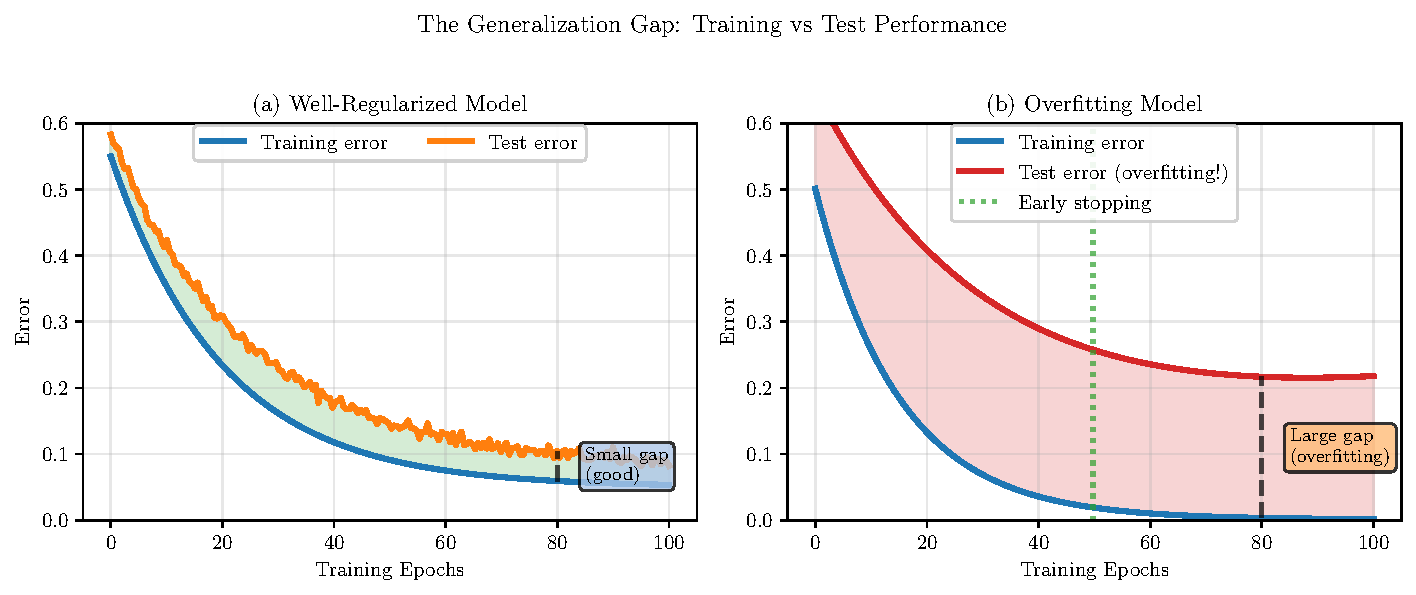
\includegraphics[width=\linewidth]{code/figures/ch09_pacbayes_mdl/fig_9_1_generalization_gap.pdf}
\caption{The generalization gap across training: left, a well-regularized model keeps test error close to training error; right, an overfitting model shows a large gap that early stopping can curb.}
\label{fig:generalization_gap}
\end{figure}

\vspace{1.5em}

\subsection{The Role of Priors and Inductive Bias}

Not all compression is equal. You could compress your training data by inventing an arbitrary code that maps each example to a short bitstring. But this code wouldn't help you compress new examples unless they happened to be in your training set. The compression that matters for generalization is compression that respects the structure of the data-generating process.

\vspace{0.3cm}

This is where priors come in. A prior distribution over models encodes your inductive bias---your beliefs about which models are more plausible before seeing any data. Simple models might get higher prior probability than complex ones. Models that respect symmetries in the problem might be favored over those that don't. The prior shapes what counts as "efficient" compression.

\vspace{0.3cm}

In the Bayesian framework, the prior $p(\theta)$ over parameters $\theta$ combines with the likelihood $p(D|\theta)$ of the data $D$ to give the posterior $p(\theta|D)$. But we can also read this through an information lens. The negative log prior $-\log p(\theta)$ is the codelength of the model under your inductive bias. The negative log likelihood $-\log p(D|\theta)$ is the codelength of the data given the model. The sum is the total description length, and finding the model that minimizes this sum is exactly maximum a posteriori (MAP) estimation.

\vspace{0.3cm}

This perspective suggests that generalization depends critically on your choice of prior. If your prior assigns high probability to models that are actually likely to generate the data, you'll generalize well. If your prior is misspecified, you might compress the training data efficiently according to your prior but fail to generalize because you've compressed in the wrong language, so to speak.

\vspace{2em}

%==========================
\section{PAC-Bayes Bounds: Generalization as Codelength}
%==========================

PAC-Bayes theory provides our first rigorous framework for connecting compression to generalization. The acronym stands for "Probably Approximately Correct Bayesian," which is a mouthful, but the core idea is elegant. Instead of analyzing a single hypothesis, we analyze a distribution over hypotheses, and we get generalization bounds that depend on the KL divergence between our learned distribution and a prior distribution.

\vspace{1em}

\subsection{The Classic PAC-Bayes Theorem}

Let me state the theorem first, then unpack what it means. Assume a bounded loss in $[0,1]$, and interpret risk for the \emph{Gibbs} predictor that samples $h \sim Q$ for each prediction. Suppose you have a prior distribution $P$ over hypotheses (models) that you choose before seeing any data. After training on a dataset $D$ of size $n$, you learn a posterior distribution $Q$ over hypotheses. For any $\delta > 0$, with probability at least $1 - \delta$ over the draw of the training data, the following holds for any choice of posterior \$Q\$ (even if \$Q\$ depends on the data):

\vspace{0.3cm}

\begin{equation}
\mathbb{E}_{h \sim Q}[\text{Risk}(h)] \leq \mathbb{E}_{h \sim Q}[\text{EmpRisk}(h)] + \sqrt{\frac{\text{KL}(Q \| P) + \log(n/\delta)}{2n}}
\end{equation}

\vspace{0.3cm}

\begin{figure}[t]
\centering
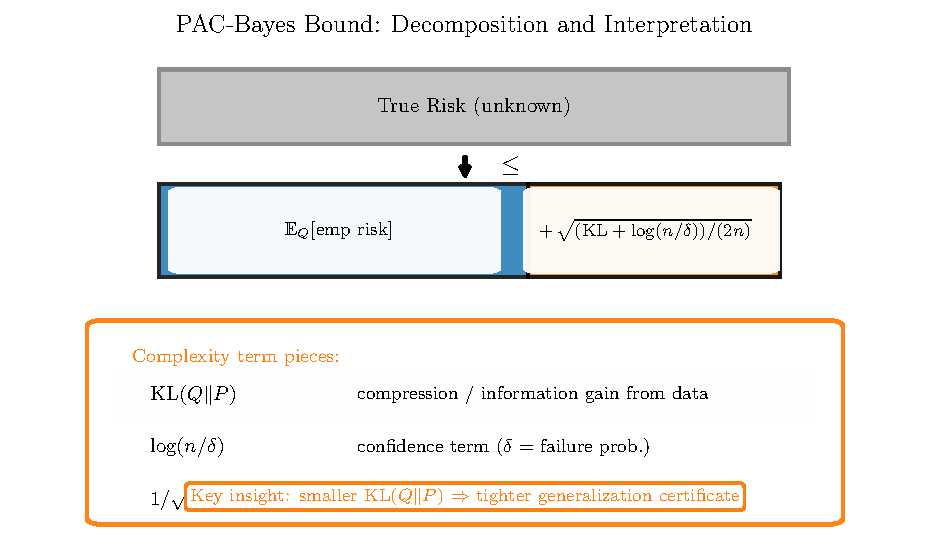
\includegraphics[width=\linewidth]{code/figures/ch09_pacbayes_mdl/fig_9_2_pacbayes_bound.pdf}
\caption{PAC--Bayes bound decomposition: true risk is upper-bounded by empirical risk plus a complexity penalty of order $\sqrt{(\mathrm{KL}(Q\|P)+\log(n/\delta))/(2n)}$.}
\label{fig:pacbayes_bound}
\end{figure}

\vspace{0.3cm}

Here, $\text{Risk}(h)$ is the true risk---the expected loss of hypothesis $h$ on new data from the data-generating distribution. $\text{EmpRisk}(h)$ is the empirical risk---the average loss on the training data. The bound says that the true risk is close to the empirical risk, with a gap that depends on the KL divergence from the posterior to the prior and the sample size.

\vspace{0.3cm}
\textit{Interpretation.} The probability is over the random draw of the training sample; the prior $P$ must be fixed before seeing the data. You are then free to pick any data-dependent posterior $Q$ and plug it into the bound. Formally, the guarantee is for the randomized Gibbs predictor; deterministic predictors or ensembling usually need extra arguments, though the bound remains a useful guide.

\vspace{0.3cm}

Let's parse this carefully. The left side is what we care about: the expected loss on new data when we sample a hypothesis from our learned distribution $Q$. The right side has two terms. The first term is the expected training loss, which we can measure directly. The second term is the generalization penalty, and it grows with the square root of the KL divergence divided by the sample size.

\vspace{0.3cm}

The KL divergence $\text{KL}(Q \| P)$ is the key quantity. From our work in earlier chapters, we know this is the extra codelength required to describe samples from $Q$ when using a code optimized for $P$. In the context of PAC-Bayes, it measures how much information we've extracted from the training data beyond what our prior already told us. If $Q$ is close to $P$, we've learned little---the KL is small, and the bound is tight. If $Q$ is far from $P$, we've learned a lot---the KL is large, and we need more data to ensure good generalization.

\vspace{1em}


\vspace{0.3cm}
\begin{keyinsight}
\textbf{Prior vs posterior in PAC\mbox{-}Bayes.} The prior $P$ must be chosen \emph{before} observing the dataset $D$, while the posterior $Q$ may depend on $D$. This mirrors Bayesian language (cf. Chapter~2) but the bound is over \emph{distributions of predictors}, not just a single model.
\end{keyinsight}

\vspace{0.3cm}
The confidence parameter $\delta$ controls the probability with which the bound holds: smaller $\delta$ (higher confidence) yields a looser bound.
\subsection{Interpreting the KL Term: Bits of Information}

Let's make the information-theoretic interpretation explicit. The KL divergence $\text{KL}(Q \| P)$ can be written as:

\vspace{0.3cm}

\begin{equation}
\text{KL}(Q \| P) = \mathbb{E}_{h \sim Q}\left[\log \frac{Q(h)}{P(h)}\right] = \mathbb{E}_{h \sim Q}[-\log P(h)] - H(Q)
\end{equation}

\vspace{0.3cm}

\begin{figure}[t]
\centering
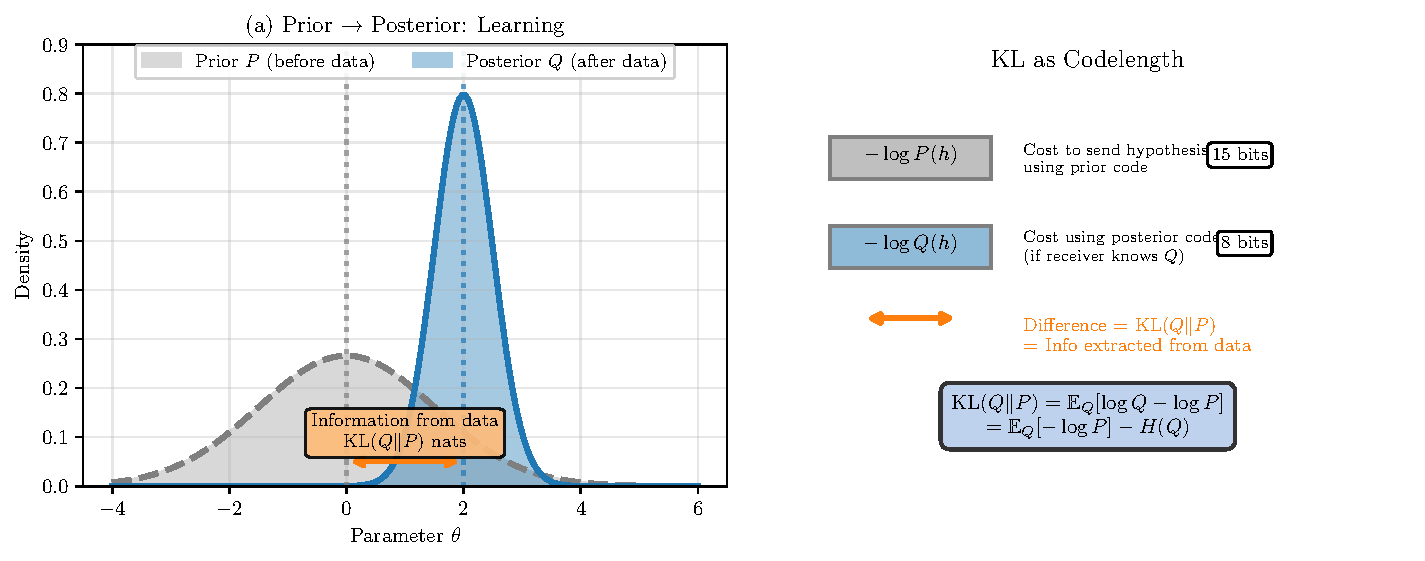
\includegraphics[width=\linewidth]{code/figures/ch09_pacbayes_mdl/fig_9_3_kl_codelength.pdf}
\caption{KL as codelength: sending hypotheses drawn from $Q$ using the prior code for $P$ wastes exactly $\mathrm{KL}(Q\|P)$ nats compared to coding with $Q$.}
\label{fig:kl_codelength}
\end{figure}

\vspace{0.3cm}

The first term, $\mathbb{E}_{h \sim Q}[-\log P(h)]$, is the expected codelength of hypotheses sampled from $Q$ under the prior code. The second term, $H(Q)$, is the entropy of the posterior distribution. If we use $Q$ to sample a hypothesis and then transmit it using the prior code, we pay an expected codelength of $\mathbb{E}_{h \sim Q}[-\log P(h)]$. But we could be more efficient: if the receiver also knows $Q$, we could use a code optimized for $Q$, paying only $H(Q)$ nats. The difference is the KL divergence.

\vspace{0.3cm}

In the PAC-Bayes setting, the KL term measures how many nats of information about the training data we've encoded into our choice of posterior. If the posterior is highly concentrated---if it puts most of its mass on a single hypothesis---then $H(Q)$ is small, and the KL is large (assuming the prior is more spread out). This makes sense: concentrating on a specific hypothesis uses up information from the training data.

\vspace{0.3cm}

Conversely, if the posterior remains broad and similar to the prior, then $H(Q)$ is large, and the KL is small. We haven't extracted much specific information from the training data, so the generalization penalty is low. This is the compression-generalization tradeoff made explicit: you can compress the training data more (concentrate the posterior) at the cost of requiring more data to guarantee generalization.

\vspace{1.5em}

\begin{examplebox}
\textbf{Worked Example: Gaussian Prior and Posterior}

Let's work through a concrete example with Gaussian distributions over a single parameter $\theta \in \mathbb{R}$. Suppose our prior is $P = \mathcal{N}(0, \sigma_P^2)$ and our posterior after training is $Q = \mathcal{N}(\mu_Q, \sigma_Q^2)$.

The KL divergence between two Gaussians has a closed form:

\begin{equation}
\text{KL}(Q \| P) = \log \frac{\sigma_P}{\sigma_Q} + \frac{\sigma_Q^2 + \mu_Q^2}{2\sigma_P^2} - \frac{1}{2}
\end{equation}

Suppose $\sigma_P = 1$ (unit variance prior), and after training we have $\mu_Q = 2$ and $\sigma_Q = 0.5$ (we've concentrated around $\theta = 2$ with half the prior variance).

The KL divergence is:

\begin{equation}
\text{KL}(Q \| P) = \log \frac{1}{0.5} + \frac{0.25 + 4}{2} - \frac{1}{2} = \log 2 + 2.125 - 0.5 \approx 2.32 \text{ nats}
\end{equation}

If we trained on $n = 1000$ examples and want confidence $\delta = 0.05$, the generalization penalty is:

\begin{equation}
\sqrt{\frac{2.32 + \log(1000/0.05)}{2 \cdot 1000}} = \sqrt{\frac{2.32 + 7.60}{2000}} \approx 0.07
\end{equation}

This tells us that with high probability, the true risk exceeds the empirical risk by at most about $0.07$ plus whatever slack comes from sampling randomness in the empirical risk itself.
\end{examplebox}

\vspace{1.5em}
\begin{pausebox}
\textbf{Reality Check: scaling to modern networks.}
The toy numbers above make the algebra tangible, but typical PAC--Bayes bounds on modern deep nets are often \emph{orders of magnitude} looser than observed test error.
When $\text{KL}(Q\|P)$ is large in absolute terms (as it often is with millions of parameters), the complexity term
$\sqrt{(\text{KL} + \log(\cdot))/(2n)}$ can dominate, yielding vacuous upper bounds (near $100\%$ risk) even when test error is small.
These bounds still provide \emph{qualitative} guidance---architectures or training procedures that reduce KL (e.g., stronger priors, weight decay, noise injections) tend to generalize better---but practitioners should not expect tight numerical certificates.
\end{pausebox}

\vspace{1.5em}



\vspace{0.3cm}
\textbf{Connection to Chapter~8.} The PAC\mbox{-}Bayes bound mirrors the VAE ELBO structure: an empirical fit term plus a KL regularizer. When the empirical risk is a log-loss, the analogy is literal; for other losses it's a structural echo. In VAEs, $\mathrm{KL}(q\|p)$ controls latent rate; in PAC\mbox{-}Bayes, $\mathrm{KL}(Q\|P)$ controls hypothesis complexity. Both express \emph{compression} governing generalization.
\subsection{From Single Hypotheses to Distributions}

One of the most powerful aspects of PAC-Bayes is that it bounds the risk of a distribution over hypotheses, not just a single hypothesis. Why is this useful? Because in practice, we often want to maintain uncertainty about which hypothesis is best, and we can exploit this uncertainty to improve performance.

\vspace{0.3cm}

When you sample a hypothesis $h$ from $Q$ and use it for prediction, you're effectively doing Bayesian model averaging at test time (the posterior predictive from Chapter~2). Different samples from $Q$ might make different predictions, and you can aggregate these predictions (by voting for classification or averaging for regression) to get better performance than any single hypothesis.

\vspace{0.3cm}

The PAC-Bayes bound applies directly to the Gibbs predictor: sampling fresh hypotheses from $Q$ for each test point. In practice, you might sample once and reuse that hypothesis, or sample multiple times and average their predictions; these often behave similarly, but the formal guarantee is for the randomized predictor. The bound tells you that the expected performance of this randomized predictor is controlled by the empirical risk and the KL divergence.

\vspace{0.3cm}

This also connects to the idea of flat minima that we'll explore in the next section. If your posterior $Q$ is broad---if it assigns significant probability to many different hypotheses---then you're less sensitive to the particular choice of hypothesis. This breadth is captured by the entropy term in the KL divergence, and it improves generalization by preventing overfitting to any single parameter setting.

\vspace{1em}


\vspace{0.3cm}
\textbf{Practical computation (one recipe).} Take $Q$ as a Gaussian centered at trained weights with covariance from a Laplace approximation (inverse Hessian or a diagonal proxy); choose $P$ as an isotropic Gaussian. This is a local quadratic approximation, not a literal Bayesian posterior, but it makes $\mathrm{KL}(Q\|P)$ analytic. In practice, many reported PAC\mbox{-}Bayes bounds remain loose by orders of magnitude; use them as \emph{qualitative} guidance.
\subsection{Choosing the Prior: Where Inductive Bias Lives}

The choice of prior $P$ is crucial for PAC-Bayes bounds. A good prior should assign high probability to hypotheses that are likely to generalize, but you have to choose the prior before seeing the training data. This is where your inductive bias---your knowledge about the problem domain---becomes mathematically formalized.

\vspace{0.3cm}

For neural networks, common choices include Gaussian priors centered at zero, which encode a preference for small parameter values. You might also use a prior centered at the parameters of a pretrained model, encoding the belief that the new task is similar to the pretraining task. The scale of the prior matters too: a broad prior (large variance) is less informative but also leads to larger KL divergence for any given posterior, while a narrow prior is more informative but requires the posterior to be very close to it to get good bounds.

\vspace{0.3cm}

There's a subtlety here that's worth noting. The prior must be chosen before seeing the test data, but it's allowed to depend on meta-knowledge about the problem class. For instance, if you know that translation invariance is important for your problem, you can build a prior that respects this symmetry. This is perfectly valid and often critical for getting useful bounds.

\vspace{0.3cm}

In practice, practitioners rarely choose priors to optimize PAC-Bayes bounds directly. Instead, they use architectural choices and regularization that implicitly define a prior. Dropout, weight decay, and data augmentation can all be interpreted as defining priors over hypotheses, and these priors affect both the KL term and the empirical risk term in the bound.

\vspace{2em}

%==========================

\vspace{0.8em}
\textbf{Bridge.} PAC-Bayes makes compression explicit via a KL term. MDL reaches the same insight from coding theory: shorter descriptions correlate with better generalization. We now rephrase the same theme in MDL's two-part code.
\vspace{0.8em}

\vspace{1em}
\textbf{Pause.} So far: generalization via PAC\mbox{-}Bayes = empirical fit plus a KL compression term. Keep this lens in mind as we switch to MDL's coding view of the same idea.
\vspace{1em}
\section{MDL: The Minimum Description Length Principle}
%==========================

We've seen how PAC-Bayes connects compression to generalization through KL divergence and priors. Now let's explore a complementary framework that makes the compression-generalization link even more direct: the Minimum Description Length (MDL) principle. MDL says, roughly, that the best model is the one that compresses the data the most.

\vspace{1em}

\subsection{Two-Part Codes and Occam's Razor}


\vspace{0.3cm}
Recall from Chapter~1: two-part MDL codes the model plus the data given the model. Here we use that lens to reason about generalization: shorter codes typically generalize better.
The MDL principle formalizes Occam's razor---the idea that simpler explanations are preferable---by measuring simplicity through codelength. The setup is elegant. Imagine you want to transmit your dataset $D$ to a receiver. You can do this in two parts:

\vspace{0.3cm}

First, you transmit a description of your model $M$. This costs $L(M)$ bits, where $L$ is some coding scheme for models. Second, you transmit the data $D$ using your model $M$ as a code. This costs $L(D|M)$ bits, which is the codelength of the data given that the receiver knows the model.

\vspace{0.3cm}

The total description length is $L(M) + L(D|M)$, and the MDL principle says you should choose the model that minimizes this sum. This trades off model complexity (the first term) against how well the model fits the data (the second term). A very complex model can fit the data perfectly, making $L(D|M)$ small, but it costs a lot to transmit the model itself. A very simple model is cheap to transmit but might not compress the data well. The best model balances these two forces.

\vspace{0.3cm}

\begin{figure}[t]
\centering
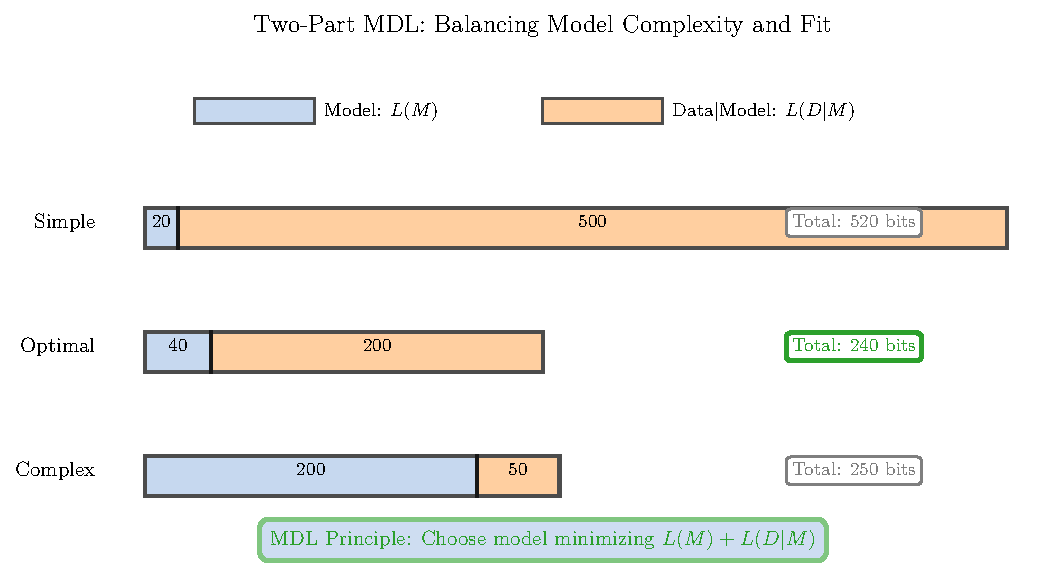
\includegraphics[width=\linewidth]{code/figures/ch09_pacbayes_mdl/fig_9_4_mdl_twopart.pdf}
\caption{Two-part MDL: total description length equals model cost $L(M)$ plus data cost $L(D\mid M)$; models that minimize the sum generalize best.}
\label{fig:mdl_twopart}
\end{figure}

\vspace{0.3cm}

Let's make this concrete with a simple example. Suppose you have a sequence of numbers: $[2, 4, 6, 8, 10, 12]$. You could transmit this as a raw list, which might cost roughly $6 \log V$ bits (where $V$ is the number of possible values). Or you could transmit the model "arithmetic sequence with start=2 and step=2" plus the data "length=6", which costs far fewer bits for the model description plus a small number of bits to specify the length. The MDL principle favors the second approach because the total codelength is lower.

\vspace{1em}



\begin{examplebox}
\textbf{Coding-scheme arbitrariness (concrete illustration).}
Consider two model families $\mathcal{M}_1$ and $\mathcal{M}_2$ that achieve the same negative log-likelihood on your data.
Under a two-part code, total description length is $L(M_i) + L(D \mid M_i)$, where $L(M_i)$ encodes the model index and its parameters.
If you choose a code that assigns a shorter description to $\mathcal{M}_1$'s parameters (e.g., quantizing weights on a hand-picked grid), you may select $\mathcal{M}_1$; a different parameter code could flip the decision.
This is not a bug, but it \emph{does} mean two-part MDL inherits a degree of design choice: the parts of the description you control can sway the outcome.
\end{examplebox}

\vspace{1.5em}
\vspace{1.5em}
\begin{examplebox}
\textbf{Worked MDL example (short).} Fit a Gaussian mean with known variance $\sigma^2$ using two models: (i) mean fixed at 0 (few bits to describe), (ii) mean free (costs $\tfrac{1}{2}\log n$ nats to encode at precision $n^{-1/2}$, the usual asymptotic cost for one free parameter). Model (ii) wins only when the reduction in negative log-likelihood exceeds this code length.
\end{examplebox}
\subsection{Connecting MDL to Maximum Likelihood}

There's a beautiful connection between MDL and probabilistic modeling. If your model assigns probability $p_M(D)$ to the data, then the optimal codelength for transmitting $D$ using $M$ is $-\log p_M(D)$ nats (or $-\log_2 p_M(D)$ bits). This is just the information-theoretic result from Chapter 1: the expected codelength under an optimal code is the entropy, and for a single data point, the codelength is the negative log probability.

\vspace{0.3cm}

So the data term $L(D|M)$ in the MDL principle corresponds to the negative log-likelihood. The model term $L(M)$ corresponds to the negative log prior probability of the model, if we have a prior distribution over models. Minimizing the total description length is therefore equivalent to maximum a posteriori (MAP) estimation:

\vspace{0.3cm}

\begin{align}
\arg\min_M [L(M) + L(D|M)] &= \arg\min_M [-\log p(M) - \log p(D|M)] \\
&= \arg\max_M [\log p(M) + \log p(D|M)] \\
&= \arg\max_M \log p(M|D)
\end{align}

\vspace{0.3cm}

This shows that MDL and Bayesian inference are deeply connected. They're both saying the same thing in different languages: the best model balances prior plausibility (model simplicity) against likelihood (fit to data). The MDL perspective makes the compression aspect explicit, while the Bayesian perspective makes the probabilistic interpretation explicit.

\vspace{1em}


\vspace{0.3cm}
\textbf{BIC as MDL.} The Bayesian Information Criterion approximates MDL under regularity by penalizing $\tfrac{k}{2}\log n$ for $k$ parameters and $n$ samples. It is the asymptotic two-part code length for parametric models with regular posteriors.
\subsection{Refined MDL and the Prequential Principle}

\begin{keyinsight}
\textbf{Why prequential MDL fixes the arbitrariness.}
Prequential (online) MDL encodes the dataset by the model's step-by-step predictive \emph{log-loss}, $\sum_{t=1}^n -\log p(x_t \mid x_{<t})$.
This codelength depends only on the model's sequential predictions, not on an external parameter code.
Different parameterizations that induce the same predictive distribution yield (up to $O(1)$ constants) the same prequential code length.
Thus, prequential MDL removes most of the coding-scheme ambiguity inherent in two-part MDL.
\end{keyinsight}

\vspace{1.2em}

\begin{examplebox}
\textbf{Mini-example.} Two parameterizations define identical predictive distributions $p_1(x\mid x_{<t}) \equiv p_2(x\mid x_{<t})$.
Two-part MDL could disagree depending on the parameter code lengths $L(M_1)$ vs $L(M_2)$.
Prequential MDL assigns both the same total codelength $\sum_t -\log p(x_t\mid x_{<t})$, sidestepping the ambiguity.
\end{examplebox}

\vspace{1.5em}


The two-part code formulation of MDL is intuitive, but it has a limitation: the model description length $L(M)$ depends on your choice of coding scheme for models, and different choices can give different answers. A more refined version of MDL, called prequential or sequential MDL, avoids this issue by considering how well your model predicts a sequence of data points.

\vspace{0.3cm}

Here's the idea. Suppose your data arrives as a sequence $x_1, x_2, \ldots, x_n$. You process it sequentially: first you see $x_1$ and make a prediction about it, then you see $x_2$ and make a prediction about it given $x_1$, and so on. Your goal is to minimize the total codelength across the sequence:

\vspace{0.3cm}

\begin{equation}
\sum_{t=1}^n L(x_t | x_1, \ldots, x_{t-1})
\end{equation}

\vspace{0.3cm}

This is called the prequential codelength because you're using your model to predict (hence "prequential," a portmanteau of "predictive" and "sequential") each data point before seeing it. If your model family is good, you'll assign high probability to each new data point given the history, resulting in short codelength. If your model family is poor, you'll be surprised by each new data point, paying a high codelength.

\vspace{0.3cm}

The beauty of this approach is that it doesn't require explicitly specifying a coding scheme for models. The model complexity is implicitly captured in how much codelength you need to specify the first few data points before your model starts making good predictions. A complex model that needs many examples to learn will pay high codelength early in the sequence, while a simple model that can generalize from few examples will achieve low codelength throughout.

\vspace{1.5em}

\begin{keyinsight}
Prequential MDL unifies compression and generalization in the most direct way possible: under an exchangeable/sequential view of the data, your ability to compress future data points given past data points is your ability to generalize. There's no separate train and test split in that setting---every data point serves as both training data (after you see it) and test data (when you're predicting it). This makes MDL a natural framework for online learning and continual learning scenarios.
\end{keyinsight}

\vspace{1.5em}


\vspace{0.3cm}
\textbf{Caution.} Short descriptions are not always better models in practice (think: Kodak held patents but missed the market). MDL is a guide, not an oracle.

\vspace{0.3cm}
Prequential (predictive) MDL codes each point using the model trained on previous data, linking description length to sequential predictive performance. We revisit this in depth in the online learning chapter; here, treat it as a refined MDL that rewards models with strong \emph{predictive} compression.
\subsection{MDL for Model Selection}

One of the most practical applications of MDL is model selection: choosing between different model families or hyperparameter settings. Classical approaches like cross-validation estimate generalization by holding out data and testing on it. MDL offers an alternative: choose the model that compresses the data the most.

\vspace{0.3cm}

For example, suppose you're deciding between a linear model and a neural network for a regression task. The linear model has few parameters and is easy to describe, so $L(M_{\text{linear}})$ is small. But it might not fit the data well if there are nonlinear patterns, so $L(D|M_{\text{linear}})$ could be large. The neural network can fit complex patterns, making $L(D|M_{\text{NN}})$ potentially small. But it has many parameters, so $L(M_{\text{NN}})$ is large.

\vspace{0.3cm}

The MDL principle says: compute the total description length for each model and pick the one with the shortest total. This automatically balances model complexity against fit, without needing to manually tune a regularization parameter. In practice, computing exact description lengths can be challenging, so practitioners often use approximations like the Bayesian Information Criterion (BIC), which is asymptotically equivalent to MDL.

\vspace{0.3cm}

There's a deep connection to generalization here. A model that compresses the training data well---achieving a short total description length---has learned a compact representation of the data's structure. This compact representation should transfer to new data from the same distribution. Conversely, a model that requires a long description length to fit the training data has probably memorized specifics rather than learning general patterns, and it will generalize poorly.

\vspace{2em}

%==========================

\vspace{0.8em}
\textbf{Bridge.} PAC\mbox{-}Bayes and MDL both say compression controls generalization. What does compression look like in parameter space? Geometry enters: flatness suggests many parameter settings yield similar predictions.
\vspace{0.8em}

\vspace{0.3cm}
\textbf{Bias--variance through compression.} The classical trade-off reappears: more complex codes reduce bias (fit) but increase variance (overfitting). Compression-oriented objectives navigate this trade-off explicitly.
\section{Flat Minima, Sharp Minima, and the Loss Landscape}
%==========================

\begin{keyinsight}
\textbf{Actionable first: train for flatness with SAM.}
The most practical takeaway from this literature is a simple optimizer modification: \emph{Sharpness-Aware Minimization (SAM)} perturbs weights in the ascent direction and then descends the worst-case loss in a small neighborhood.
In practice, SAM often improves generalization with a modest compute overhead and no architectural changes.
\end{keyinsight}

\begin{figure}[t]
\centering
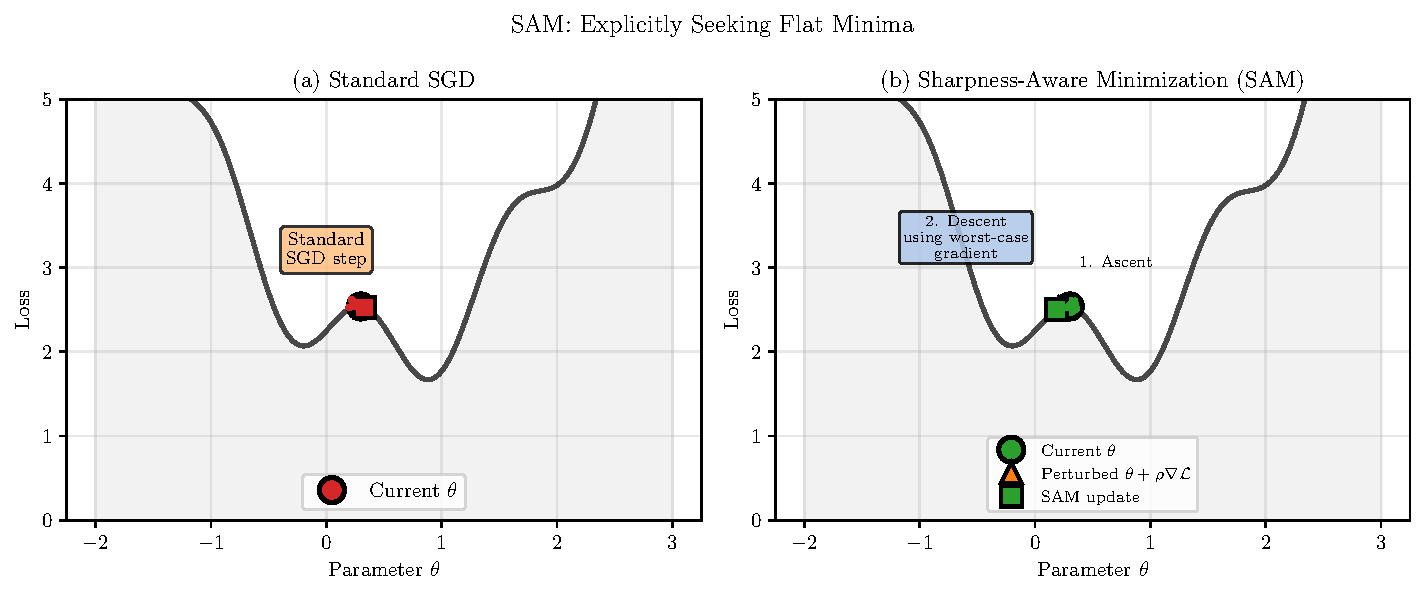
\includegraphics[width=\linewidth]{code/figures/ch09_pacbayes_mdl/fig_9_11_sam.pdf}
\caption{Sharpness-Aware Minimization (SAM): a two-step update (ascent to the worst-case neighborhood then descent) explicitly discourages sharp minima and favors flatter basins.}
\label{fig:sam}
\end{figure}

\vspace{0.8em}

Let's shift our geometric lens to the parameter space of neural networks. When you train a network, you're searching for parameters that minimize loss on your training data. But the loss landscape---the function that maps parameters to loss---has rich structure, and this structure turns out to be intimately connected to generalization.

\vspace{1em}

\subsection{Visualizing Flatness and Sharpness}

Imagine you've trained a neural network and found parameters $\theta^*$ that achieve low training loss. Now imagine perturbing these parameters slightly: $\theta^* + \epsilon \nu$ where $\nu$ is a random direction and $\epsilon$ is a small scalar. What happens to the training loss?

\vspace{0.3cm}

If the loss remains low for a wide range of perturbations, we say $\theta^*$ lies in a flat minimum. The loss landscape around $\theta^*$ looks like a broad valley. If the loss increases rapidly for small perturbations, we say $\theta^*$ lies in a sharp minimum. The loss landscape looks like a narrow spike.

\vspace{0.3cm}

Here's the key observation often reported: flat minima are often observed to generalize better than sharp minima. This is a useful heuristic, but it depends on how flatness is measured (see the caveat below). A parameter setting that's robust to perturbations on the training set is also more likely to perform well on the test set. Conversely, a parameter setting that's highly sensitive to perturbations has probably fit idiosyncrasies of the training data that won't transfer.

\vspace{0.3cm}

Let me build intuition for why this is true. Suppose you have two parameter settings that both achieve zero training loss. The first is in a flat region---you can wiggle the parameters substantially without increasing loss. The second is in a sharp region---even tiny changes increase loss dramatically. Which one do you trust to generalize?

\vspace{0.3cm}

\begin{figure}[t]
\centering
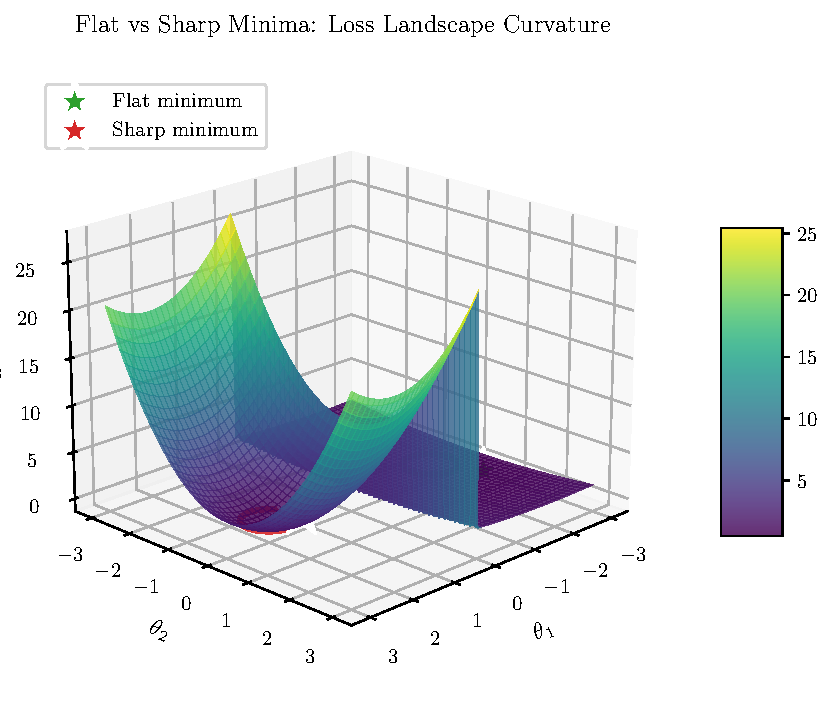
\includegraphics[width=\linewidth]{code/figures/ch09_pacbayes_mdl/fig_9_5_flat_sharp_minima.pdf}
\caption{Flat vs.\,sharp minima in a toy landscape: wide valleys are robust to perturbations, while narrow spikes are highly sensitive.}
\label{fig:flat_sharp_minima}
\end{figure}

\vspace{0.3cm}

The flat minimum is safer because it's making less specific commitments. Many nearby parameter settings also work well on the training data, which suggests that the solution isn't finely tuned to idiosyncrasies of those particular examples. The sharp minimum, by contrast, relies on precise parameter values, which is a red flag for overfitting. You've tuned the parameters so carefully that even small changes break the solution, suggesting you've fit noise rather than signal.

\vspace{1em}



\begin{keyinsight}
\textbf{Lottery tickets as MDL.} The lottery ticket hypothesis says large nets contain much smaller subnetworks that train to comparable accuracy.
From an MDL perspective, the \emph{effective} description length counts the subnetwork (plus its index), not the full parameter tensor.
Compression-aware selection therefore aligns with pruning and sparsity.
\end{keyinsight}

\vspace{1.2em}
\vspace{1.5em}
\begin{examplebox}
\textbf{Toy flatness visualization.} Consider $L(w_1,w_2)=\tfrac{1}{2}(10^2 w_1^2 + 1\cdot w_2^2)$. Contours are highly elongated: sharp along $w_1$, flat along $w_2$. A reparameterization $\tilde w_1 = 10 w_1$ makes the level sets spherical---illustrating that naive ``sharpness'' depends on parameterization.
\end{examplebox}
\subsection{Quantifying Flatness: The Hessian}


\vspace{0.3cm}
\textbf{Caveat: flatness depends on parameterization.} Naive sharpness measures are not invariant to reparameterizations: rescaling layers can make any minimum appear flatter or sharper (Dinh et al., 2017). Meaningful flatness should be defined relative to a justified parameterization or normalized by a metric like the Fisher information (natural-gradient geometry).
How do we measure flatness quantitatively? The standard approach uses the Hessian matrix---the matrix of second derivatives of the loss with respect to the parameters. At a minimum $\theta^*$, the Hessian $H = \nabla^2 \mathcal{L}(\theta^*)$ captures the local curvature of the loss landscape.

\vspace{0.3cm}

If the eigenvalues of $H$ are all small, the minimum is flat---the loss doesn't increase much as you move away from $\theta^*$ in any direction. If some eigenvalues are large, the minimum is sharp---the loss increases rapidly along the corresponding eigenvectors. The trace of $H$, which sums the eigenvalues, is one way to quantify overall sharpness, while the largest eigenvalue quantifies the sharpest direction.

\vspace{0.3cm}

For neural networks, computing the full Hessian is expensive---it's a matrix of size $d \times d$ where $d$ is the number of parameters, and $d$ can be in the billions. But we can approximate it using various techniques: stochastic estimates, power iteration to find the largest eigenvalues, or diagonal approximations that capture the per-parameter curvature.

\vspace{0.3cm}

Another approach is to define flatness through perturbations directly. The sharpness can be measured as:

\vspace{0.3cm}

\begin{equation}
\text{Sharpness}(\theta^*) = \max_{\|\epsilon\| \leq r} \mathcal{L}(\theta^* + \epsilon) - \mathcal{L}(\theta^*)
\end{equation}

\vspace{0.3cm}

This asks: within a ball of radius $r$ around $\theta^*$, how much can the loss increase? A flat minimum has low sharpness because the loss stays nearly constant within the ball. A sharp minimum has high sharpness because the loss can increase substantially even within a small neighborhood.

\vspace{1em}

\begin{geometrylens}
The loss landscape of a neural network is a high-dimensional geometric object, and minima are points where the gradient vanishes. The Hessian at a minimum defines a local quadratic approximation to the landscape, and its eigenvalues describe the principal curvatures. Flat minima correspond to regions where the manifold is nearly level in many directions, while sharp minima are isolated points where the manifold curves steeply.
\end{geometrylens}

\begin{figure}[t]
\centering
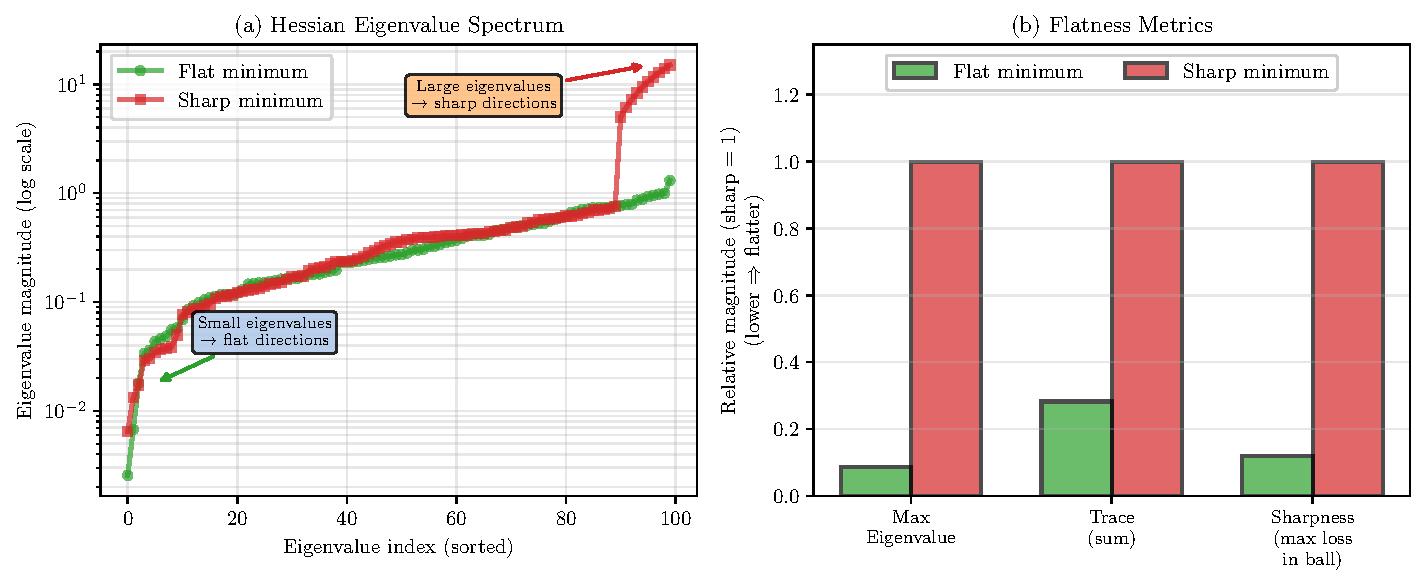
\includegraphics[width=\linewidth]{code/figures/ch09_pacbayes_mdl/fig_9_6_hessian_flatness.pdf}
\caption{Hessian-based diagnostics: sharp minima exhibit large leading eigenvalues and higher sharpness metrics; flatter minima have smaller spectra and lower values.}
\label{fig:hessian_flatness}
\end{figure}


\vspace{0.3cm}
\textbf{How to measure (and how hard is it?).}
Exact Hessians are intractable for modern nets. Practical surrogates include: (i) top eigenvalue via power/Lanczos iterations on Hessian--vector products (cost: a handful of data passes); (ii) Hutchinson trace estimates for $\mathrm{tr}(H)$ (cost: a few backprop-like probes); and (iii) \emph{sharpness} proxies that measure loss increase under small, norm-bounded parameter perturbations (used by SAM).
For large vision models, these range from minutes to hours on a single GPU; full spectra are out of reach (days to weeks).

\vspace{0.8em}

\begin{keyinsight}
\textbf{Flatness depends on parameterization; use an invariant metric.}
"Sharpness" measured in raw parameters can be made arbitrarily large or small by simple rescalings of layers, so it is not an intrinsic notion.
A principled alternative is to measure curvature in a parameterization-invariant geometry, such as the Fisher information metric (natural gradient view).
Qualitative takeaway: prefer measures tied to predictive change, not raw weight scales.
\end{keyinsight}

\vspace{1.2em}
\vspace{1.5em}

\subsection{Connecting Flatness to PAC-Bayes}

Now comes the beautiful connection: flat minima have a natural PAC-Bayes interpretation, and this interpretation makes the generalization advantage precise. Suppose your prior $P$ is a Gaussian centered at some initialization $\theta_0$, and your posterior $Q$ is a Gaussian centered at the trained parameters $\theta^*$ with covariance $\Sigma$.

\vspace{0.3cm}

The KL divergence between these Gaussians depends on both how far $\theta^*$ is from $\theta_0$ and how the covariance $\Sigma$ relates to the prior covariance. If you choose $\Sigma$ to match the inverse Hessian---so that the posterior is broader in flat directions and narrower in sharp directions---then the KL term naturally penalizes sharp minima more than flat ones.

\vspace{0.3cm}

Here's why. If $\theta^*$ is in a sharp minimum, the Hessian has large eigenvalues, so the inverse Hessian has small eigenvalues. A Gaussian with covariance equal to the inverse Hessian would be very narrow in the sharp directions, meaning it's concentrated tightly around $\theta^*$. This concentration costs information---the KL divergence from a narrow posterior to a broad prior is large.

\vspace{0.3cm}

Conversely, if $\theta^*$ is in a flat minimum, the Hessian has small eigenvalues, so the inverse Hessian has large eigenvalues. The corresponding Gaussian posterior is broad, and if the prior is also reasonably broad, the KL divergence is smaller. Less information is needed to specify a flat minimum because many nearby parameters work equally well.

\vspace{0.3cm}

\begin{figure}[t]
\centering
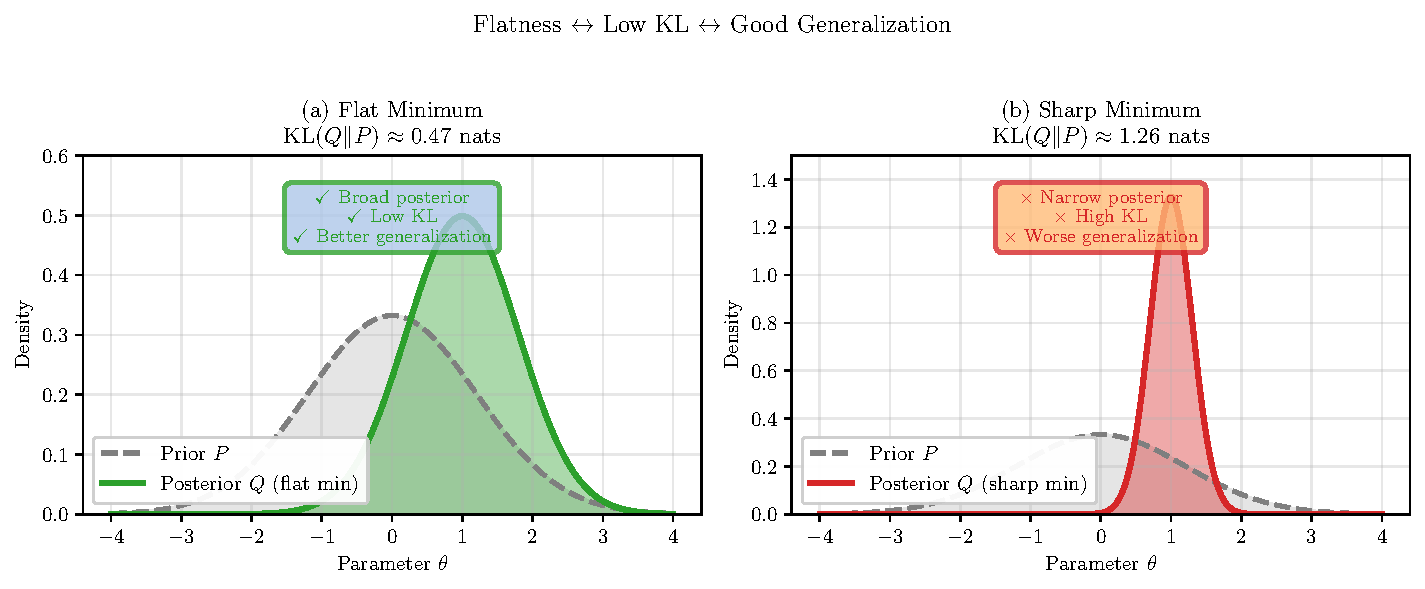
\includegraphics[width=\linewidth]{code/figures/ch09_pacbayes_mdl/fig_9_7_flatness_pacbayes.pdf}
\caption{Flatness \textrightarrow{} low KL in PAC--Bayes: broad posteriors around flat minima incur smaller $\mathrm{KL}(Q\|P)$ than narrow posteriors needed at sharp minima.}
\label{fig:flatness_pacbayes}
\end{figure}

\vspace{0.3cm}

This connection suggests an algorithm: explicitly optimize the PAC-Bayes bound during training by maintaining a posterior distribution that balances low empirical risk against low KL divergence to the prior. This is exactly what techniques like stochastic weight averaging, Gaussian posterior approximations (like in the Laplace approximation), and certain forms of Bayesian deep learning try to do.

\vspace{1em}


\vspace{0.3cm}
\textbf{From theory to practice: SAM.} Sharpness\mbox{-}Aware Minimization perturbs parameters to penalize nearby loss increases, explicitly biasing toward flatter minima. Empirically it often improves robustness and generalization, making the flatness lens actionable.
\subsection{Why SGD Finds Flat Minima}

Here's a fascinating empirical observation: when you train neural networks with stochastic gradient descent, especially with small batch sizes and moderate learning rates, you tend to find flat minima. Why should this be true? The optimizer isn't explicitly seeking flatness---it's just following (noisy) gradients toward low loss.

\vspace{0.3cm}

The key is the noise in the gradient estimates. When you compute gradients on a minibatch rather than the full dataset, you get a noisy estimate of the true gradient. This noise acts as implicit regularization, effectively preventing the optimizer from converging to sharp minima. Here's the intuition: a sharp minimum is a small target. The noise in SGD makes it hard to stay precisely at a sharp minimum---you keep getting kicked out of it by stochastic fluctuations. A flat minimum, by contrast, is a large target. Once you enter a flat region, the noise is less likely to push you out because there's a whole neighborhood of low-loss parameters.

\vspace{0.3cm}

This can be formalized through the lens of stochastic differential equations. In the continuous-time limit, SGD with learning rate $\eta$ and batch size $b$ follows a gradient flow with noise proportional to $\eta/b$. In steady state, this process samples from a distribution that assigns higher probability to flatter minima. The noise causes the optimizer to explore around minima, and flat minima have larger basins of attraction in this noisy process.

\vspace{0.3cm}

\begin{figure}[t]
\centering
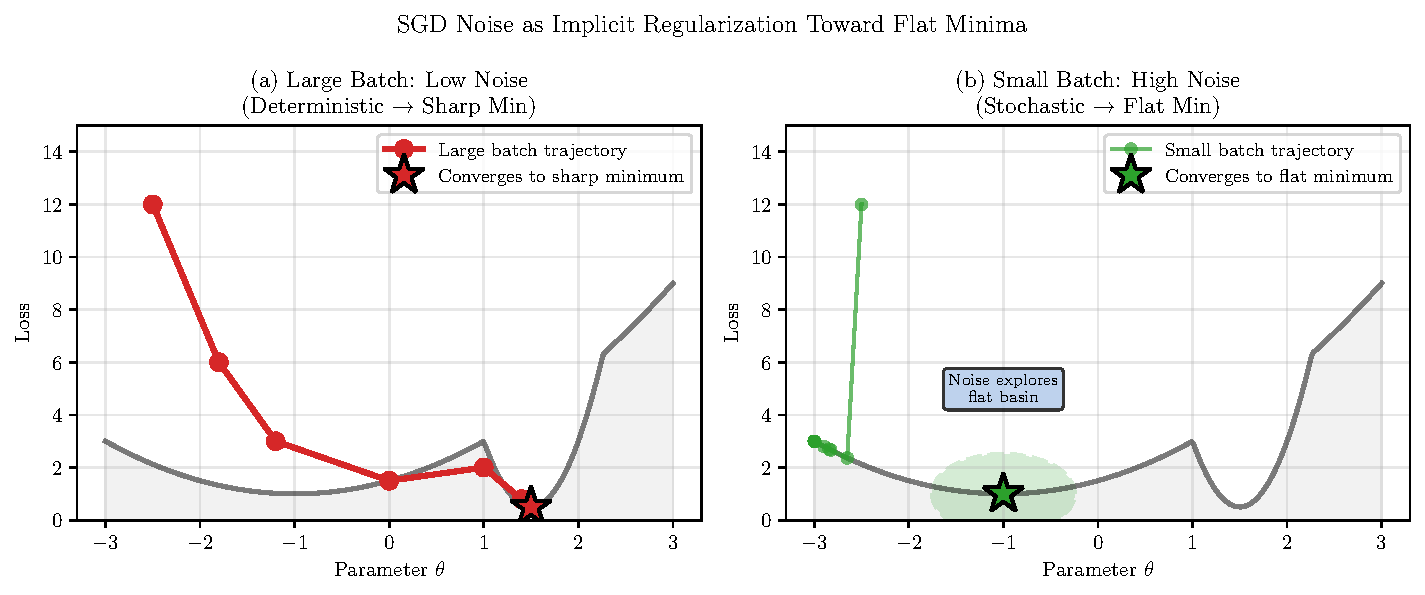
\includegraphics[width=\linewidth]{code/figures/ch09_pacbayes_mdl/fig_9_8_sgd_noise.pdf}
\caption{SGD noise as implicit regularization: high noise explores and settles in flat basins, while low noise trajectories can converge to sharp minima.}
\label{fig:sgd_noise}
\end{figure}

\vspace{0.3cm}

This also explains why large batch training sometimes hurts generalization. With very large batches, the gradient estimates are nearly deterministic, reducing the noise that implicitly regularizes toward flat minima. To compensate, practitioners often need to add explicit regularization or use learning rate schedules that maintain some level of noise throughout training.

\vspace{2em}

%==========================

\vspace{1em}
\textbf{Pause.} PAC\mbox{-}Bayes, MDL, and flatness tell one story: compression $\leftrightarrow$ generalization. Next: when not to predict at all---selective prediction.
\vspace{1em}

\vspace{0.3cm}
Whether SGD inherently prefers flat minima remains debated; measurement artifacts may confound the effect. Treat flatness as a useful lens, not a settled law.

\vspace{0.3cm}
\textbf{A cautious view.} One proposed explanation models SGD as a stochastic differential equation whose stationary distribution favors wide basins.
Another connects overparameterized networks to kernel regression in the Neural Tangent Kernel (NTK) regime, where implicit bias selects minimum-norm (hence smoother) solutions.
Both stories have empirical support in restricted settings, but the general claim that SGD inherently prefers flat minima remains \emph{actively debated}. Treat these as useful intuitions, not laws.

\begin{keyinsight}
\textbf{Double descent through the compression lens.}
Test error can first rise near interpolation and then fall again as parameters grow (``double descent'').
From an MDL/PAC--Bayes perspective, larger models may discover \emph{shorter effective codes} (e.g., via sparse subnetworks or flatter, more compressible solutions), even as raw capacity increases.
This reconciles overparameterization with generalization: capacity enables search; compression explains success.
\end{keyinsight}

\vspace{1.2em}
\section{Selective Prediction and Risk Control}
%==========================

\noindent\emph{Why here?}
Selective prediction is about \textbf{information triage}: deciding when the model has enough bits of evidence to make a reliable prediction.
It closes the loop between compression (\S9.1) and guarantees (\S9.2): we trade coverage for risk, allocating our model's limited predictive capacity where it matters most.

\vspace{0.8em}

All the theory we've developed so far assumes that our model makes a prediction for every input. But there's a powerful alternative: sometimes the model should abstain from predicting when it's uncertain. This is called selective prediction, and it connects beautifully to the information-theoretic framework we've been building.

\vspace{1em}

\subsection{The Risk-Coverage Tradeoff}

Selective prediction introduces a new degree of freedom: the model can choose not only what to predict but also when to predict. Formally, a selective predictor consists of a prediction function $f(x)$ and a selection function $g(x) \in \{0, 1\}$ that indicates whether to predict (1) or abstain (0).

\vspace{0.3cm}

The goal is to achieve low risk on the inputs where we do predict, while maintaining reasonable coverage---the fraction of inputs for which we make predictions. There's an obvious tradeoff: if we only predict on the easiest examples, we can achieve very low risk but poor coverage. If we predict on everything, we get full coverage but higher risk. The challenge is to navigate this tradeoff optimally.

\vspace{0.3cm}

Let's make this quantitative. Define the selective risk as the expected loss on the points where we predict:

\vspace{0.3cm}

\begin{equation}
R_{\text{sel}}(f,g) = \mathbb{E}[\ell(f(x), y) \cdot g(x) \mid g(x) = 1]
\end{equation}

\vspace{0.3cm}

And define the coverage as:

\vspace{0.3cm}

\begin{equation}
\text{Cov}(g) = \mathbb{E}[g(x)]
\end{equation}

\vspace{0.3cm}

For any desired level of coverage $c \in (0,1]$, we want to find the selection function that minimizes selective risk while achieving at least coverage $c$. Intuitively, we should predict on the inputs where we're most confident and abstain on the ones where we're uncertain.

\vspace{1em}

\subsection{Using Model Confidence for Selection}

The natural approach to selective prediction is to use the model's own confidence as a signal for when to abstain. For a classifier, this might be the maximum predicted probability. For a regressor, this might be the predictive variance. The selection function becomes:

\vspace{0.3cm}

\begin{equation}
g(x) = \mathbb{1}[\text{confidence}(x) \geq \tau]
\end{equation}

\vspace{0.3cm}

where $\tau$ is a threshold chosen to achieve the desired coverage. By varying $\tau$, we trace out a risk-coverage curve: as coverage increases, risk typically increases too because we're including more uncertain predictions.

\vspace{0.3cm}

\begin{figure}[t]
\centering
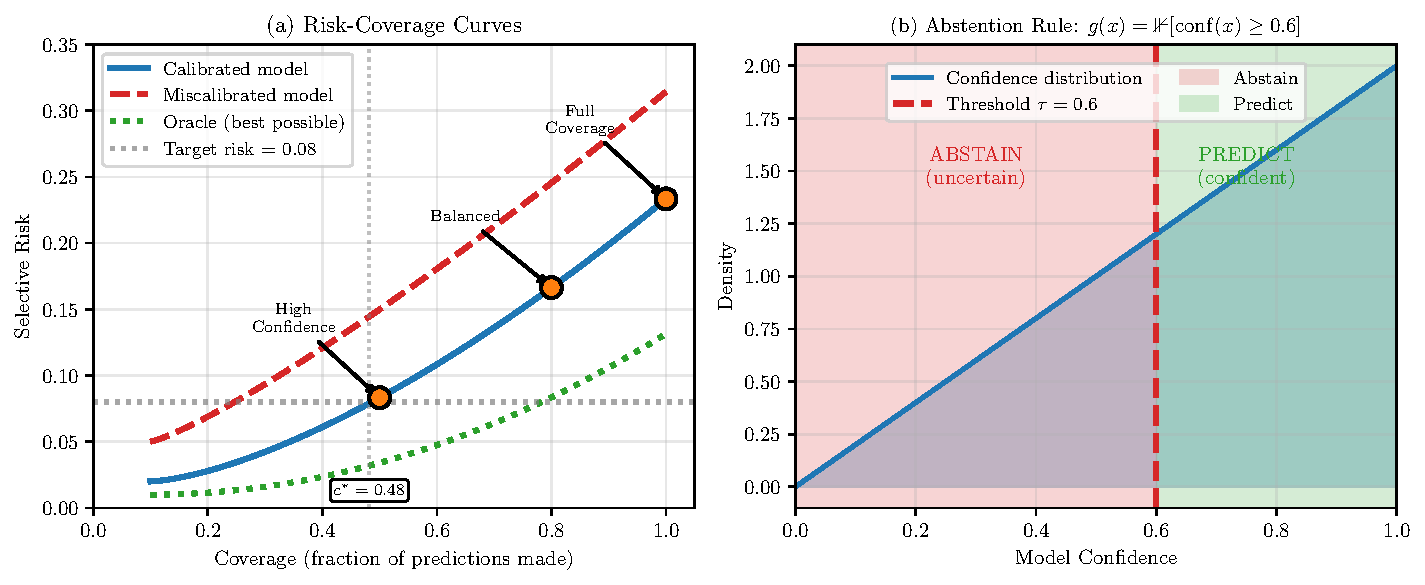
\includegraphics[width=\linewidth]{code/figures/ch09_pacbayes_mdl/fig_9_9_risk_coverage.pdf}
\caption{Selective prediction: (a) risk--coverage curves illustrate the tradeoff; (b) an abstention rule accepts predictions only when confidence exceeds a threshold.}
\label{fig:risk_coverage}
\end{figure}

\vspace{0.3cm}

But there's a catch. The model's confidence might be miscalibrated---the predicted probabilities might not match the true frequencies. An overconfident model assigns high probability to predictions that are often wrong, leading to poor selective risk even when predicting only on high-confidence examples. This is where calibration, which we discuss further in Chapter 13 (Calibration), becomes critical.

\vspace{0.3cm}

There's also a connection to the information budgeting framework that we'll develop in Chapter 14 (Information Budgeting). Abstention is a way of saying "I don't have enough information to make this prediction reliably." By declining to predict, we're acknowledging that the expected utility of making a prediction is negative---the risk of being wrong exceeds the benefit of being right, given our uncertainty.

\vspace{1em}

\subsection{PAC-Bayes Bounds for Selective Prediction}
The abstention setting changes the denominator: you only incur risk on the \emph{covered} subset. We therefore need bounds that control the true selective risk as a function of the number of covered points $n_c$, not the full sample size $n$. PAC--Bayes extends naturally: replace the empirical/true risks with their selective counterparts and scale the complexity penalty by $1/n_c$.

\vspace{0.3cm}

PAC-Bayes theory extends naturally to the selective prediction setting, giving us rigorous guarantees on the risk-coverage tradeoff. As before, assume bounded loss, and let the selection depend only on inputs (or confidence), not labels. The key modification is that we now bound the selective risk conditional on the selection function, rather than the unconditional risk.

\vspace{0.3cm}

Here's a simplified version of the bound. For a prior $P$, posterior $Q$, and selection function $g$ with coverage $c$ (the fraction selected on the sample), we have with high probability:

\vspace{0.3cm}

\begin{equation}
R_{\text{sel}}(f,g) \leq \text{EmpRisk}_{\text{sel}}(f,g) + \sqrt{\frac{\text{KL}(Q \| P) + \log(n/\delta)}{2nc}}
\end{equation}

\vspace{0.3cm}

Notice the critical difference: the sample size in the denominator is now $nc$ rather than $n$. This makes sense---if you're only predicting on a fraction $c$ of the data, you effectively have fewer samples to learn from for those predictions. The bound gets tighter as coverage increases because you have more data to bound the risk on.

\vspace{0.3cm}

This bound gives us a principled way to choose the coverage level. If we're deploying a model in a safety-critical setting, we might require that the selective risk be below some threshold $r^*$ with high confidence. The bound tells us how much we need to shrink the coverage to guarantee this risk level, given our empirical performance and the KL divergence of our model.

\vspace{1em}

\begin{examplebox}
\textbf{Worked Example: Setting Coverage for a Target Risk}

Suppose we've trained a binary classifier and obtained a posterior $Q$ with $\text{KL}(Q \| P) = 3$ nats. On our training set of $n=10000$ examples, we observe an empirical selective risk of $0.02$ at coverage $c=0.5$ (predicting on the top 50\% most confident examples).

Using the PAC-Bayes bound with $\delta = 0.05$, the generalization penalty is:

\begin{equation}
\sqrt{\frac{3 + \log(10000/0.05)}{2 \cdot 10000 \cdot 0.5}} = \sqrt{\frac{3 + 10.6}{10000}} \approx 0.037
\end{equation}

So we can be 95\% confident that the true selective risk is at most $0.02 + 0.037 = 0.057$.

If our target risk is $0.05$, we're not quite there at $c=0.5$. We need to reduce coverage. Suppose at $c=0.3$, the empirical selective risk drops to $0.01$. The penalty becomes:

\begin{equation}
\sqrt{\frac{13.6}{6000}} \approx 0.048
\end{equation}

giving a total bound of $0.01 + 0.048 = 0.058$, still slightly above target.

At $c=0.2$, with empirical risk $0.005$, we get:

\begin{equation}
\sqrt{\frac{13.6}{4000}} \approx 0.058
\end{equation}

for a total of $0.063$. It looks like we need to go even lower in coverage or gather more data to reliably hit our target risk of 0.05.
\end{examplebox}

\vspace{1.5em}


\vspace{0.3cm}
\textbf{Caveat.} Selection must depend only on features $x$ (or model confidence) at test time. If $g(x)$ peeks at labels $y$, bounds with denominator $n_c$ no longer apply.
\subsection{Conformal Prediction: Distribution-Free Guarantees}

PAC-Bayes bounds require assumptions about the data distribution and the model family. An alternative framework called conformal prediction provides distribution-free guarantees for selective prediction. The core idea is simple but powerful: you can construct a prediction set that's guaranteed to contain the true label with probability at least $1 - \alpha$, for any choice of $\alpha$, without making any assumptions about the data distribution.

\vspace{0.3cm}

Here's how it works. You hold out a calibration set---a set of labeled examples that you don't use for training. For each possible label $y$, you compute a nonconformity score that measures how unusual it would be for that example to have label $y$. You then rank the calibration examples by their nonconformity scores.

\vspace{0.3cm}

At test time, for a new input $x$, you compute the nonconformity score for each possible label. You include label $y$ in your prediction set if its nonconformity score is less than or equal to the $(1-\alpha)$ quantile of the calibration scores. By construction, this procedure guarantees that the prediction set contains the true label with probability at least $1 - \alpha$, assuming the calibration and test points are i.i.d. (equivalently, exchangeable draws from the same distribution).

\vspace{0.3cm}

\begin{figure}[t]
\centering
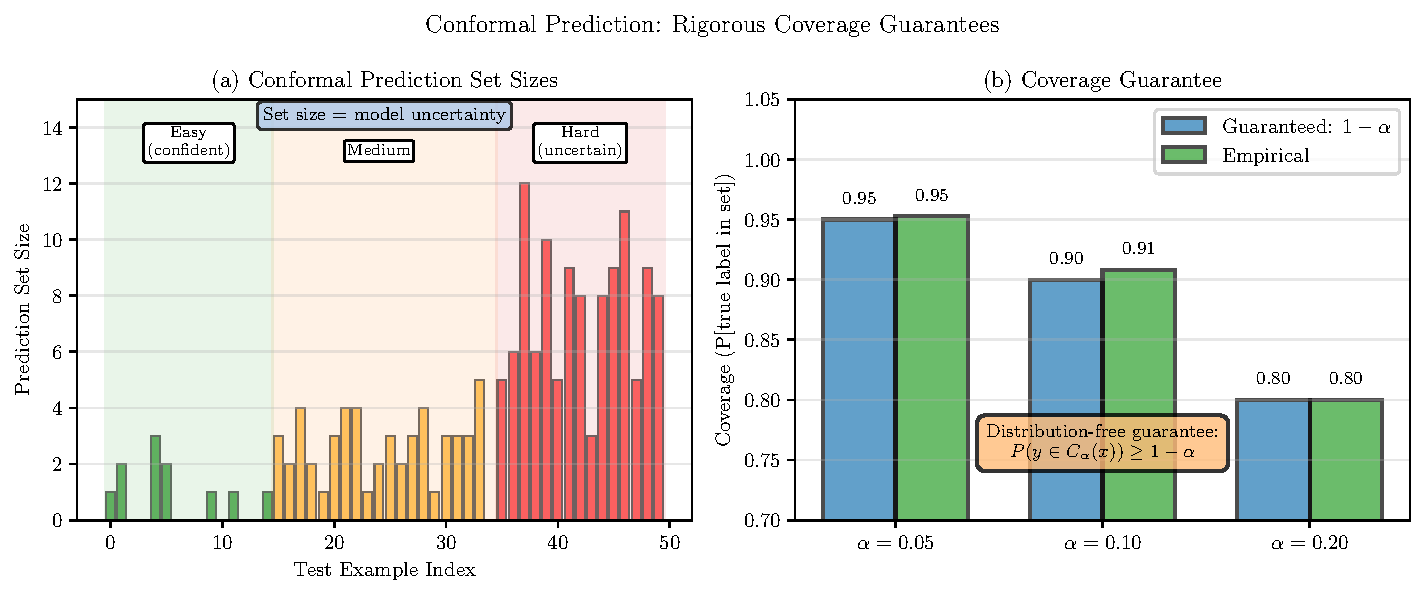
\includegraphics[width=\linewidth]{code/figures/ch09_pacbayes_mdl/fig_9_10_conformal_prediction.pdf}
\caption{Conformal prediction: set sizes reflect uncertainty (left) and empirical coverage tracks the guaranteed $1-\alpha$ levels (right) under the IID assumption.}
\label{fig:conformal_prediction}
\end{figure}

\vspace{0.3cm}

The connection to selective prediction comes through the size of the prediction set. When the model is confident, the prediction set will be small---often just a single label. When the model is uncertain, the prediction set will be large, possibly including many labels. You can use the prediction set size as a signal for selective prediction: only make a definite prediction when the conformal set is small, and abstain when it's large.

\vspace{0.3cm}

Conformal prediction is appealing for generative models and structured outputs, where traditional calibration methods can be difficult to apply, though set sizes can be large and guarantees are typically marginal. We'll return to this theme in Chapter 13 when we discuss calibration for language models and other generative systems.

\vspace{2em}

%==========================

\section{Exercises}

\begin{enumerate}
\item \textbf{Compute a PAC--Bayes bound.} For a binary classifier with $n=10{,}000$, empirical error $\hat{L}=0.05$, prior $P=\mathcal{N}(0,I)$, posterior $Q=\mathcal{N}(\mu,\sigma^2 I)$ with $\text{KL}(Q\|P)=250$, evaluate a standard PAC--Bayes bound at $\delta=0.05$.
\item \textbf{KL between Gaussians.} Derive the KL for (a) diagonal-covariance Gaussians and (b) full-covariance Gaussians, and compare magnitudes for the same mean shift.
\item \textbf{Implement a selective predictor.} Using any trained classifier, implement abstention via a confidence threshold. Plot risk--coverage curves before and after temperature scaling.
\item \textbf{Measure sharpness.} Estimate the top Hessian eigenvalue of a trained network using power iteration on Hessian--vector products. Compare to a SAM-trained version.
\end{enumerate}

\vspace{1.5em}

\section{Practical Implications for Model Training}

\begin{itemize}
\item \textbf{Do not over-interpret PAC--Bayes numerically.} Use PAC--Bayes as a \emph{qualitative} guide to favor priors/posteriors that compress (small KL). Bounds on modern nets are typically loose.
\item \textbf{Track compression proxies during training.} Monitor the KL term when available (e.g., variational training), weight norms, or a sharpness proxy (e.g., SAM objective gap). Rising complexity without validation gains is a warning sign.
\item \textbf{Use flatness-aware optimization when generalization matters.} SAM is a low-friction default; start with small $\rho$ (perturbation radius) and compare validation curves.
\item \textbf{When (not) to compute bounds.} Exact Hessians are $O(d^2)$ to store and impractical; top-eigen estimates and diagonal/low-rank approximations are cheap(er) sanity checks. Computing full PAC--Bayes certificates is rarely worthwhile in production, but can be useful for comparative studies.
\item \textbf{Risk--coverage curves for high-stakes settings.} Implement selective prediction with a simple confidence threshold; plot empirical risk vs coverage and choose an operating point that meets domain constraints. Calibrate first (Chapter 13 (Calibration)).
\end{itemize}

\vspace{1.2em}
\section{Chapter Summary and Looking Forward}
%==========================

This chapter has woven together several threads connecting compression, generalization, and prediction under uncertainty. Let's gather what we've learned and see how it prepares us for the chapters ahead.

\vspace{0.3cm}

PAC-Bayes theory makes precise the intuition that compression enables generalization. The KL divergence from posterior to prior measures how many nats of information we've extracted from the training data, and this quantity appears in generalization bounds that control the gap between training and test performance. Models that compress efficiently---that achieve low empirical risk with small KL divergence---come with tighter bounds and are expected to generalize better under the same distributional assumptions.

\vspace{0.3cm}

The geometry of the loss landscape offers a lens on why flat minima often generalize better than sharp ones. Flat minima correspond to broad posterior distributions with low KL divergence, while sharp minima correspond to concentrated posteriors with high KL divergence. Stochastic gradient descent can bias training toward flatter regions through gradient noise, providing a plausible algorithmic explanation for why standard training procedures often generalize well.

\vspace{0.3cm}

The Minimum Description Length principle reformulates learning as compression: the best model is the one that compresses the data the most, balancing model complexity against fit through a two-part code. Prequential MDL makes this even more direct in sequential settings by equating compression ability with predictive accuracy on sequential data. This framework unifies many model selection criteria and provides a clear information-theoretic objective for learning.

\vspace{0.3cm}

Selective prediction extends our framework to scenarios where abstention is an option. PAC-Bayes bounds for selective risk show how coverage affects the sample complexity required for guarantees, while conformal prediction provides distribution-free coverage guarantees through calibration sets. These tools are essential for deploying models in settings where reliability requirements are paramount.

\vspace{0.3cm}

\begin{figure}[t]
\centering
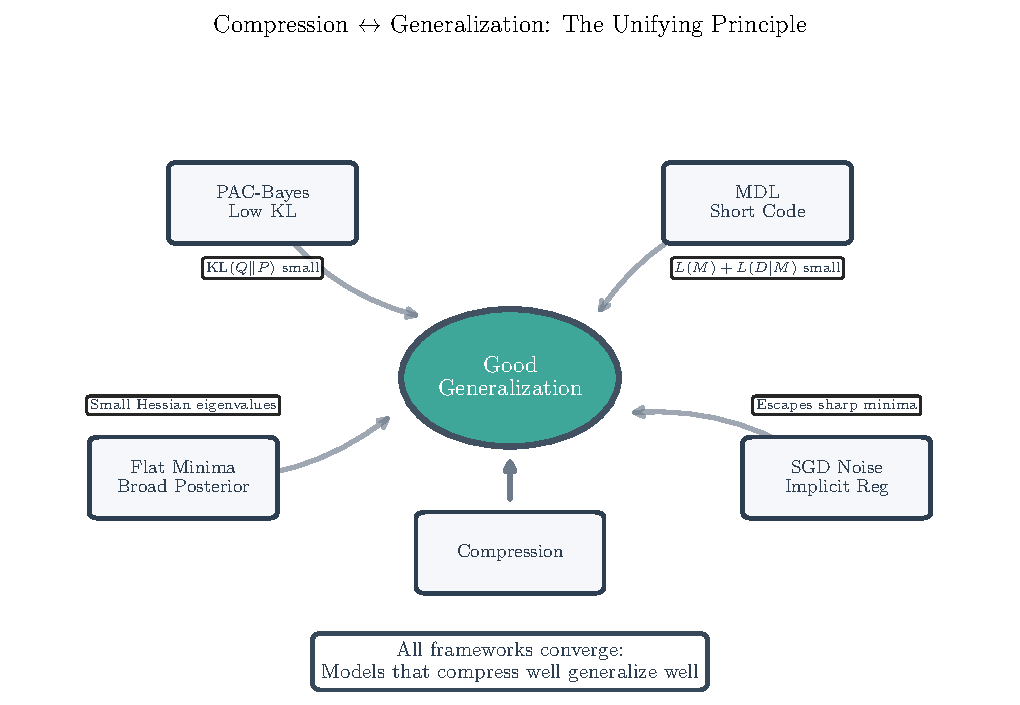
\includegraphics[width=\linewidth]{code/figures/ch09_pacbayes_mdl/fig_9_12_unifying_view.pdf}
\caption{A unifying view: PAC--Bayes (low KL), MDL (short codes), flat minima (small Hessian), and SGD noise all align with the principle that better compression tends to align with better generalization.}
\label{fig:unifying_view}
\end{figure}

\vspace{0.3cm}

In the next chapter, we'll turn to scaling laws---the empirical regularities that govern how model performance improves with more compute, data, and parameters. The compression framework developed here will help us understand why these scaling laws exist and how to navigate the tradeoffs between different resources. We'll see that scaling is ultimately about allocating information capacity efficiently, and the geometric and information-theoretic tools we've built will illuminate the structure of these allocation problems.

\vspace{1em}

\begin{pausebox}
\textbf{Key Takeaways from Chapter 9}

Compression and generalization are fundamentally linked through information theory. PAC-Bayes bounds show that models with low KL divergence from prior to posterior tend to generalize better, formalizing Occam's razor through codelength. Flat minima in the loss landscape correspond to broad posteriors and are often associated with good generalization, while sharp minima correspond to narrow posteriors and overfitting. MDL provides an alternative formulation where the best model minimizes total description length. Selective prediction uses compression ideas to decide when to abstain, with PAC-Bayes and conformal prediction providing rigorous risk-coverage guarantees. All these frameworks share a common language: generalization as compression is a useful lens, and good models are efficient compressors.
\end{pausebox}
